\documentclass[a4paper,10pt]{article}

% Packages
% -------------------- %

% Apply the document encoding
\usepackage[utf8]{inputenc}
% Set the document language/s
\usepackage[english]{babel}
% Set margins
\usepackage[hmargin=2cm,vmargin=3cm,headheight=16pt]{geometry}
% Apply the Merryweather font
\usepackage{merriweather}
\usepackage[T1]{fontenc}
% Customize links
\usepackage[english]{hyperref}
% Include graphics
\usepackage{graphicx}
% Create better tables
\usepackage{tabularx}
% Use floating positioning (like H inside figures)
\usepackage{float}
% Customize lists
\usepackage{enumitem}
% Customize the line height
\usepackage{setspace}
% Customize the space between paragraphs
\usepackage{parskip}
% Provide additional color syntax
\usepackage{xcolor}
% Customize headers and footers
\usepackage{fancyhdr}
% Create cells inside tables
\usepackage{makecell}
% Customize section style
\usepackage{titlesec}

% Package config
% -------------------- %

% Set line height
\setstretch{1.2}
% Remove indent for the first paragraph line
\setlength{\parindent}{0pt}
% Set space between paragraphs
\setlength{\parskip}{6pt}

% Remove table cell padding
\renewcommand{\tabcolsep}{1pt}

% Customize link colors
\hypersetup{
  colorlinks=true,
  linkcolor=black,
  filecolor=black,
  urlcolor=black,
  citecolor=black
}
\urlstyle{same}

% Use dashes for itemize
\renewcommand\labelitemi{-}

% Remove space between itemize elements and decrease the left margin
\setlist[itemize]{nosep,leftmargin=*}

% Set graphics folder path
\graphicspath{{./img/}}

% Heading color
\definecolor{sky}{HTML}{2079C7}

% Setup page styles

% Page number only
\fancypagestyle{style1}{
  \fancyhf{}
  \renewcommand{\headrulewidth}{0pt}
  \fancyfoot[R]{\thepage}
}

% Name and page number
\fancypagestyle{style2}{
  \fancyhf{}
  \renewcommand{\headrulewidth}{0pt}
  \fancyhead[R]{\name}
  \fancyfoot[R]{\thepage}
}

% Hide section numbers without breaking everything
\renewcommand\thesection{}
\makeatletter
\def\@seccntformat#1{\csname #1ignore\expandafter\endcsname\csname the#1\endcsname\quad}
\let\sectionignore\@gobbletwo
\let\latex@numberline\numberline
\def\numberline#1{\if\relax#1\relax\else\latex@numberline{#1}\fi}
\makeatother

% Setup section style
\titleformat{\section}[hang]
  {\sffamily\bfseries\color{sky}}{\thesection}{0em}{\MakeUppercase}

\newcommand{\name}{Gianni Tumedei}

\renewcommand{\title}[1]{{\huge \textbf{#1}}}

\renewcommand{\section}[1]{{\sffamily
  \vspace{10pt}
  \textcolor{sky}{\textbf{\expandafter\MakeUppercase\expandafter{#1}}}
  \vspace{20pt}
}}

\newcommand{\heading}[1]{{\large \textbf{#1} \vspace{4pt}}}

\newcommand{\subheading}[1]{\textit{#1}\newline}

\newcommand{\twocols}[2]{
  \begin{tabularx}{\textwidth}{ p{0.3\textwidth} X p{0.65\textwidth} }
    \makecell[tl]{#1} && #2 \\
  \end{tabularx}
  \vspace{20pt}
}

\input{env}

% -------------------- %

\begin{document}

\pagestyle{style1}

% -------------------- %

\twocols{
  \raisebox{\dimexpr-\height+\baselineskip}{
    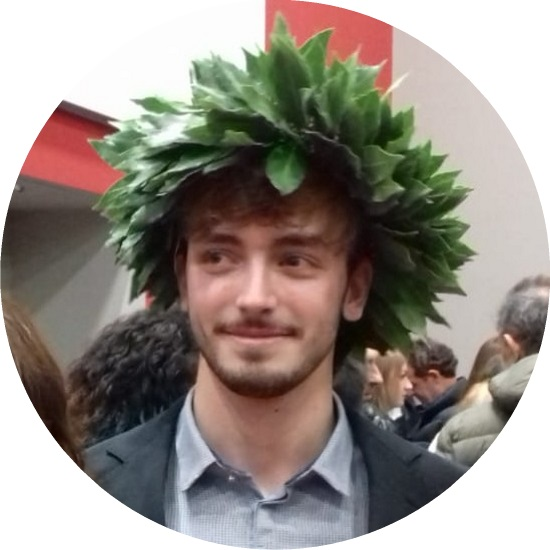
\includegraphics[width=0.3\textwidth,height=0.3\textwidth]{profile3_round.jpg}
  }
}{
  \title{\name}\newline
  {\begin{tabularx}{0.65\textwidth}{ p{1cm} X }
    \iconrow{
      
\includegraphics[width=0.5cm]{email-outline.png}
    }{
      \email{\emaila} \newline \email{\emailb} \newline \email{\emailc} \vspace{10pt}
    }
    \iconrow{
      
\includegraphics[width=0.5cm]{phone-outline.png}
    }{
      \tel{\phone} \vspace{10pt}
    }
    \iconrow{
      
\includegraphics[width=0.5cm]{web.png}
    }{
      \link{\website}{\website} \vspace{10pt}
    }
    \iconrow{
      
\includegraphics[width=0.5cm]{map-marker-outline.png}
    }{
      \address \vspace{10pt}
    }
    \iconrow{
      
\includegraphics[width=0.5cm]{account-outline.png}
    }{
      Birth date: \birthdate \newline Citizenship: \citizenship
    }
  \end{tabularx}}
}

% -------------------- %

\section{Current Occupation}

Teaching tutor at the University of Bologna, campus of Cesena, for the courses of
\begin{itemize}
  \item Web Services and Applications (Applicazioni e Servizi Web) of the second cycle degree in Computer Science and Engineering (Ingegneria e Scienze Informatiche)
  \item Web Systems Engineering (Ingegneria dei Sistemi Web) of the first cycle, career-oriented degree in Computer Systems Technologies (Tecnologie dei Sistemi Informatici)
\end{itemize}

\vspace{20pt}

% -------------------- %

\section{Work Experience}

\twocols{
  2022 - Today
}{
  \heading{University of Bologna}\newline
  \subheading{Teaching Tutor}

  \textbf{Subject}: Web Services and Applications (Applicazioni e Servizi Web)\newline
  \textbf{Course}: second cycle degree in Computer Science and Engineering (Ingegneria e Scienze Informatiche)
}

\twocols{
  2022 - Today
}{
  \heading{University of Bologna}\newline
  \subheading{Teaching Tutor}

  \textbf{Subject}: Web Systems Engineering (Ingegneria dei Sistemi Web)\newline
  \textbf{Course}: first cycle degree in Computer Systems Technologies (Tecnologie dei Sistemi Informatici)\newline
  \textbf{Tasks}:
  \begin{itemize}
    \item Hold lectures
    \item Support in laboratory lectures
    \item Correction of exam projects
  \end{itemize}
}

\twocols{
  2022
}{
  \heading{University of Bologna}\newline
  \subheading{Teaching Tutor}

  \textbf{Subject}: Foundations of Web Systems (Fondamenti di Sistemi Web)\newline
  \textbf{Course}: first cycle degree in Computer Systems Technologies (Tecnologie dei Sistemi Informatici)\newline
  \textbf{Tasks}:
  \begin{itemize}
    \item Support in laboratory lectures
    \item Correction of exam projects
  \end{itemize}
}

% Make sure this gets rendered on page 2
\pagestyle{style2}

\twocols{
  October - December 2021
}{
  \heading{Scientific High School “Augusto Righi”, Cesena (FC)}\newline
  \subheading{Computer Science and Technology Teacher}

  \textbf{Tasks}:
  \begin{itemize}
    \item Substitute teacher in the subject of Computer Science
    \item Support for foreign students in learning the italian language and studying Computer Science
  \end{itemize}
}

\twocols{
  May - September 2021
}{
  \heading{University of Bologna -Navile Project}\newline
  \subheading{Contract for research activity}

  Development, for the new Navile building complex of the University of Bologna, of an intuitive and usable wayfinding platform that provides public kiosk displays with a responsive UI, SVG maps and indications on how to reach campus spaces.\newline

  \textbf{Supervisor}: Prof. Catia Prandi\newline
  \textbf{Research team}: two researchers of the Computer Science and Engineering department, two research students\newline
  \textbf{Technologies}: Node.js, TypeScript, Vue.js, Express, MySQL
}

\twocols{
  2021
}{
  \heading{Morethantech}\newline
  \subheading{Web developer}

  Creation and maintenance of the Morethantech website (\link{https://morethantech.it}{https://morethantech.it}).\newline

  \textbf{Technologies}: Node.js, TypeScript, Vue.js, tRPC, MySQL, Docker.
}

\twocols{
  December 2020 - February 2021
}{
  \heading{University of Lisbon - Maré Project}\newline
  \subheading{Scholarship for research activities}

  Development of a platform to help students return to normal after Covid-19, by offering a ML predicted value of the number of people inside campus spaces, a feedback system to improve estimates, and an unenforced booking system, all accessible via a mobile application.\newline

  \textbf{Supervisors}: Prof. Catia Prandi, Prof. Augusto Esteves\newline
  \textbf{Research team}: international team with members from the University of Bologna, University of Minho, University of Porto, ITI / LARSyS, University of Lisbon\newline
  \textbf{Technologies}: Dart, Flutter, Google Maps SDK, Firebase\newline
  \textbf{Related publications}:
  \begin{itemize}
    \item Crowdsensing-enabled Service Design for Floating Students during the COVID-19 Pandemic
    \item Promoting a Safe Return to University Campuses during the COVID-19 Pandemic: Crowdsensing Room Occupancy
  \end{itemize}
}

\twocols{
  October - November 2019
}{
  \heading{Tajana, Barlocco, Galluccio \& Partners}\newline
  \subheading{Web developer}

  Creation of a website for the company (\link{https://tbgstudio.it}{https://tbgstudio.it}).\newline

  \textbf{Technologies}: HTML, CSS, JavaScript, Bootstrap, PHP.
}

\twocols{
  April 2018
}{
  \heading{Infia S.r.l.}\newline
  \subheading{Occasional performance}

  VBA macro programming in Microsoft Excel.
}

\twocols{
  October 2016 - July 2017
}{
  \heading{Infia S.r.l.}\newline
  \subheading{Employment - IT support}

  \textbf{Activities and responsibilities}:
  \begin{itemize}
    \item Supporting the IT manager
    \item Troubleshooting, maintenance and system integration and configuration tasks
    \item Collaboration in the migration project towards ERP and MES systems, with particular regard to data migration
    \item Collaboration in the project for the installation of an automatic palletizer in one of the company's production departments
    \item IT assistance to employees
    \item Employees workstation setup
    \item VBA macro programming in Microsoft Excel
    \item Queries on SQL Server Management Studio
    \item Product label design using ZPL language
  \end{itemize}
}

\twocols{
  February - July 2016
}{
  \heading{Infia S.r.l.}\newline
  \subheading{Internship - IT support}

  \textbf{Activities and responsibilities}:
  \begin{itemize}
    \item Supporting the IT manager in various troubleshooting, maintenance and system integration and configuration tasks
    \item IT assistance to employees
    \item Employees workstation setup
    \item VBA macro programming in Microsoft Excel
    \item Queries on SQL Server Management Studio
  \end{itemize}
}

\twocols{
  June - July 2014
}{
  \heading{Infia S.r.l.}\newline
  \subheading{Internship in collaboration with ITT B. Pascal}

  \textbf{Activities and responsibilities}:
  \begin{itemize}
    \item Supporting the IT manager
    \item IT assistance to employees
    \item VBA macro programming in Microsoft Excel
    \item Queries on SQL Server Management Studio
  \end{itemize}
}

\twocols{
  July 2013, July - August 2012
}{
  \heading{eSTATE ATTIVI project - ITAS G. Garibaldi Cesena}\newline
  \subheading{Volunteering il collaboration with the Municipality of Cesena}

  Sale of the company's fruit products.
}

% -------------------- %

\section{Education and Qualifications}

\twocols{
  2019 - 2022
}{
  \heading{Second cycle degree in Computer Science and Engineering}\newline
  \subheading{University of Bologna, Campus of Cesena}

  \textbf{Grade}: 110/110 and honors\newline
  \textbf{Class n.}: LM-32 Computer systems engineering\newline
  \textbf{Elaborate details}:
  \begin{itemize}
    \item[] \textbf{Title}: Towards a Smart Campus Digital Twin: Promoting Awareness and Sustainability Through Wayfinding and Real-Time Environmental Data
    % TODO: add description
    \item[] \textbf{Subjects}: Web Services and Applications
    \item[] \textbf{Supervisor}: Prof. Catia Prandi
  \end{itemize}
}

\twocols{
  2015 - 2019
}{
  \heading{First cycle degree in Computer Science and Engineering}\newline
  \subheading{University of Bologna, Campus of Cesena}

  \textbf{Grade}: 100/110\newline
  \textbf{Class n.}: L-8 Information technology engineering\newline
  \textbf{Elaborate details}:
  \begin{itemize}
    \item[] \textbf{Title}: Il protocollo OPC UA
    \item[] \textbf{Description}: Detailed analysis of the OPC Unified Architecture protocol, an open source and cross platform solution for data exchange in the industrial and IoT fields.
    \item[] \textbf{Supervisor}: Prof. Franco Callegati
    \item[] \textbf{Subject}: Telecommunication Networks
    \item[] \textbf{URL}: https://amslaurea.unibo.it/19780/
  \end{itemize}
}

\twocols{
  2010 - 2015
}{
  \heading{High school graduation in Computer Science and Telecommunications}\newline
  \subheading{Istituto Tecnico Tecnologico Statale Blaise Pascal - P.le Macrelli, 100 - 47521 Cesena (FC)}

  \textbf{Grade}: 100/100\newline
  \textbf{Address subjects}:
  \begin{itemize}
    \item Computer technology
    \item Systems and Networks
    \item Project Management and Business Organization
    \item Electronics and Telecommunications
    \item Systems Technology \& Design
  \end{itemize}
}

\twocols{
  2015
}{
  \heading{First Certificate in English (FCE)}\newline
  \subheading{Istituto Tecnico Tecnologico Statale Blaise Pascal - P.le Macrelli, 100 - 47521 Cesena (FC)}

  \textbf{Grade}: A\newline
  \textbf{Level}: C1\newline
  \textbf{Certification body}: Cambridge English Language Assessment
}

\twocols{
  2015
}{
  \heading{Garden in-depth and excellence course}\newline
  \subheading{Istituto Tecnico Tecnologico Statale Blaise Pascal - P.le Macrelli, 100 - 47521 Cesena (FC)}

  Creation of a greenhouse equipped with an online data acquisition and consultation system.
}

\twocols{
  2014
}{
  \heading{Basic training course for workers}\newline
  \subheading{Istituto Tecnico Tecnologico Statale Blaise Pascal - P.le Macrelli, 100 - 47521 Cesena (FC)}

  Training on:
  \begin{itemize}
    \item Concepts of risk, damage, prevention, protection
    \item Rights and duties of the various company subjects
    \item Mechanical, electrical, chemical, carcinogenic, biological risks
    \item Workplaces, VDTs, work stress
    \item Signs, emergencies
    \item Safety and first aid procedures
    \item Accidents and injuries
  \end{itemize}
}

\twocols{
  2013
}{
  \heading{Preliminary English Test (PET)}\newline
  \subheading{Istituto Tecnico Tecnologico Statale Blaise Pascal - P.le Macrelli, 100 - 47521 Cesena (FC)}

  \textbf{Level}: B2\newline
  \textbf{Certification body}: Cambridge English Language Assessment
}

\twocols{
  2010
}{
  \heading{Key English Test (KET)}\newline
  \subheading{University of Bologna, Campus of Cesena}

  \textbf{Level}: A2\newline
  \textbf{Certification body}: Cambridge English Language Assessment
}

% -------------------- %

\section{Publications}

\twocols{
  November 6 2021
}{
  \heading{Crowdsensing-enabled Service Design for Floating Students during the COVID-19 Pandemic}\newline
  \subheading{Shuhao Ma, Valentina Nisi, Augusto Esteves, Catia Prandi, Hugo Nicolau, Gianni Tumedei, João Nogueira, Francesco Boschi, and Nuno Jardim Nunes}

  In Proceedings of the 9th Congress of the International Association of Societies of Design Research (IASDR '21).\newline

  \link{https://doi.org/10.1007/978-981-19-4472-7_61}{https://doi.org/10.1007/978-981-19-4472-7\_61}
}

\twocols{
  September 9 2021
}{
  \heading{Promoting a Safe Return to University Campuses during the COVID-19 Pandemic: Crowdsensing Room Occupancy}\newline
  \subheading{Gianni Tumedei, Francesco Boschi, Catia Prandi, Luìs Gomes, Rui Calheno, Rui Abreu, Shuhao Ma, Valentina Nisi, Nuno Nunes, Augusto Esteves}

  In Proceedings of the Conference on Information Technology for Social Good (GoodIT '21).\newline

  \link{https://doi.org/10.1145/3462203.3475911}{https://doi.org/10.1145/3462203.3475911}
}

\twocols{
  December 12 2019
}{
  \heading{Il protocollo OPC UA}\newline
  \subheading{Gianni Tumedei, Franco Callegati (supervisor)}

  \link{https://amslaurea.unibo.it/19780}{https://amslaurea.unibo.it/19780}
}

% -------------------- %

\section{Awards and Acknowledgements}

\twocols{
  2021
}{
  \heading{OSM11 Hackfest - Winner}\newline
  \subheading{Team Asterisk Unibo: Onur Ozenir, Gianni Tumedei, Gyordan Caminatti, Luca Salvigni, Mattia Rossi}

  Exploiting OpenStack, Juju Charms and Asterisk for the implementation and deployment of a Virtual Network Function for VoIP calls.\newline

  \link{https://osm.etsi.org/wikipub/index.php/OSM11_Hackfest}{https://osm.etsi.org/wikipub/index.php/OSM11\_Hackfest}
}

\twocols{
  2014
}{
  \heading{IT Olympics - Territorial selection}\newline
  \subheading{Istituto Tecnico Tecnologico Statale Blaise Pascal - P.le Macrelli, 100 - 47521 Cesena (FC)}

  Participation to the territorial selection of the Italian IT Olympics and the related training course.
}

% -------------------- %

\section{Scientific Conferences}

\twocols{
  July 10-13 2022
}{
  \heading{IEEE International Conference on Distributed Computing Systems (ICDCS 2022)}\newline
  \subheading{Volunteer}
}

\twocols{
  September 9-11 2021
}{
  \heading{ACM International Conference on Information Technology for Social Good (GoodIT 2021)}\newline
  \subheading{Speaker}

  \textbf{Track title}: Promoting a Safe Return to University Campuses during the COVID-19 Pandemic: Crowdsensing Room Occupancy
}

% -------------------- %

\section{Volunteering}

\twocols{
  2018 - Today
}{
  \heading{AVIS Cesena}\newline
  \subheading{Blood donor}
}

% -------------------- %

\section{Skills}

\twocols{Mother language}{\heading{Italian}}

\twocols{Other languages}{
  \heading{English}\newline
  Level: C1\newline\newline

  \heading{Spanish}\newline
  Level: A1
}

\twocols{
  Programming skills
}{
  \heading{Programming languages}

  {\begin{tabularx}{0.65\textwidth}{ X X X }
    \begin{itemize}
      \item TypeScript
      \item JavaScript
      \item Python
      \item PHP
      \item Go
    \end{itemize}
    &
    \begin{itemize}
      \item Java
      \item Scala
      \item Kotlin
      \item Visual Basic
    \end{itemize}
    &
    \begin{itemize}
      \item Dart
      \item C
      \item C++
      \item C\#
    \end{itemize}
  \end{tabularx}}

  \heading{Markup languages and other DSLs}

  {\begin{tabularx}{0.65\textwidth}{ X X X }
    \begin{itemize}
      \item HTML
      \item CSS
      \item SCSS
    \end{itemize}
    &
    \begin{itemize}
      \item SQL
      \item GraphQL
    \end{itemize}
    &
    \begin{itemize}
      \item Markdown
      \item LaTeX
    \end{itemize}
  \end{tabularx}}

  \heading{Technologies and frameworks}

  {\begin{tabularx}{0.65\textwidth}{ X X X }
    \begin{itemize}
      \item Node.js
      \item Vue.js
      \item React
      \item SolidJS
    \end{itemize}
    &
    \begin{itemize}
      \item Svelte
      \item Electron
      \item Spring Boot
      \item Flutter
    \end{itemize}
    &
    \begin{itemize}
      \item Git
      \item Docker
      \item MongoDB
    \end{itemize}
  \end{tabularx}}
}

\twocols{Driving licence}{B}

\twocols{Other skills}{Amateur football player}

\end{document}